\documentclass{beamer}
\usepackage[utf8]{inputenc}
% \usepackage[english]{babel}
\usepackage{hyperref}
\usepackage{graphicx}
\graphicspath{{../../output/figures/Presentation/}}
\usepackage{wrapfig}
\usepackage{subcaption}
\usepackage{booktabs,bbm}
% \usepackage[square,numbers]{natbib}
%\bibliographystyle{unsrtnat}

\makeatletter
\let\@@magyar@captionfix\relax
\makeatother
\newtheorem{defn}[theorem]{Definition}
\DeclareMathOperator*{\argmax}{arg\,max}
\DeclareMathOperator*{\argmin}{arg\,min}
\hypersetup{
    colorlinks=true,
    linkcolor=blue,
    filecolor=magenta,      
    urlcolor=cyan,
}

\usetheme{Boadilla}
\usecolortheme{beaver}

\usepackage[
backend=biber,
style=bwl-FU,
sorting=ynt
]{biblatex}
\addbibresource{../main.bib}

\title[Agricultural Index Insurance]{Agricultural Index Insurance: An Optimization Approach}
\author[José I. Velarde Morales]{José I. Velarde Morales}
\institute[Chicago Booth]
{

  University of Chicago\\
  Booth School of Business

}


  


\begin{document}
\frame{\titlepage}
\section{Introduction}

\subsection{The Problem of Agricultural Risk}
\begin{frame}{The Problem of Agricultural Risk}
\begin{itemize}
    \setlength\itemsep{2em}
    \item Farmers face a lot of risk, and the lack of risk management tools forces them to use coping strategies that hurt their long term welfare.
   
    \item Traditional insurance is prohibitively costly in most developing countries due to lack of data and high verification costs.

    \item Moral hazard, adverse selection, and the presence of large covariate shocks make the problem of agricultural insurance especially hard. 
\end{itemize}
\end{frame}

\subsection{A Proposed Solution: Index Insurance}
\begin{frame}{A Proposed Solution: Index Insurance}
\begin{itemize}
   \setlength\itemsep{1em}
    \item Researchers developed index insurance as a less costly way to offer insurance in developing countries. 
    \item In index insurance, an index (or statistic) is created using easily observable quantities (e.g. rainfall), and it is used to determine whether the insured party suffered an adverse event. 
    \item If the index falls below a pre-determined threshold, the insurance company automatically issues out payments to the insured. 
    \item This allows the insurance company to circumvent the issue of verification and moral hazard, since the actions of individual farmers cannot affect the index.
\end{itemize}
\end{frame}

\begin{frame}{Index Insurance in Practice}
\begin{itemize}
    \setlength\itemsep{1.5em}
    \item Since it was first proposed, index insurance programs have been implemented in many countries including India, Mexico, Tanzania, Malawi, Kenya, and many others (\cite{jensen2017agricultural}). 
    
    \item Today, tens of millions of farmers worldwide are covered by index insurance programs (\cite{greatrex2015scaling}). 
    
    \item However, in most of these cases, the insurance has to be heavily subsidized by governments due to high cost and low demand (\cite{greatrex2015scaling}). 
\end{itemize}
\end{frame}

\subsection{Project Overview}
\begin{frame}{Project Overview}
 \begin{itemize}
    \setlength\itemsep{1em}
     \item The goal of this project is to make insurance less costly by improving the design of the insurance contracts. 
    \item Traditionally, the contract for each insured zone is designed independently of all other zones. %This ignores valuable information about the correlation between zones that affects the cost of insuring the whole portfolio. 
    \item Our method simultaneously determines the contract parameters for different areas, while taking into account the correlation between the areas. 
    \item This allows it to make better trade offs between coverage and the costs associated with capital requirements.
 \end{itemize}
\end{frame}

\begin{frame}{What I would like feedback on}
    \begin{itemize}
       \setlength\itemsep{1em}
        \item Evaluation (what metrics to report, evaluation with observational and synthetic data, etc.)
       \item Data imputation
    \end{itemize}
   \end{frame}

% \subsection{Literature Review}
\begin{frame}{Index Insurance Literature}
 \begin{itemize}
     \item \textbf{Impact of Index Insurance:} Overall, there is evidence that index insurance reduces reliance on detrimental risk-coping strategies, increases investment, and leads to riskier, but more profitable production decisions (\cite{jensen2017agricultural};  \cite{cole2013barriers}; \cite{mobarak2013informal}; \cite{karlan2014agricultural}).
     \item \textbf{Demand for Index Insurance:} Demand for index insurance tends to be low and highly price sensitive (\cite{jensen2017agricultural};  \cite{cole2013barriers}; \cite{cai2020subsidy},\cite{casaburi2018time}).
     \item \textbf{Design of Index Insurance:} There has been relatively little research studying the design of index insurance. The method developed by \cite{chantarat2013designing} is the most commonly used in academic publications (\cite{jensen2019does};  \cite{flatnes2018improving}).
 \end{itemize}
\end{frame}

% \begin{frame}{Optimization Literature}
%  \begin{itemize}
%     \setlength\itemsep{2em}
%      \item We draw from the literature on chance constrained programs (\cite{lagoa2005probabilistically}; \cite{charnes1958cost}).
%      \item  We also draw on the work on coherent risk measures (\cite{artzner1999coherent}), and work on the optimization of conditional value at risk by (\cite{rockafellar2000optimization})
     
%      \item Additionally, we use the results on convex approximations of chance constrained programs by (\cite{nemirovski2007convex}).
%  \end{itemize}
% \end{frame}



\section{Optimization Approach}
\begin{frame}[noframenumbering, plain]
    \frametitle{Content}
    \tableofcontents[currentsection]
  \end{frame}

  
\subsection{Index Insurance Background}
\begin{frame}{Index Insurance: General Context}
\begin{itemize}
    \setlength\itemsep{1em}
    \item Index insurance is a named-peril insurance.
    \item It is often tied to access to credit.
    \item Offered at different levels (micro level, meso level, and macro level)
    \item Often based on public-private partnerships. Research institutions usually design the product, and insurance companies (or governments) sell it. 
\end{itemize}
\end{frame} 

\begin{frame}{Index Insurance: Design}
Index insurance design generally consists of three steps: 
\begin{enumerate}
    \setlength\itemsep{1em}
    \item Prediction: building a model to predict loss. 
    \item Contract design: designing contracts specifying payouts based on model predictions.
    \item Pricing: product pricing
\end{enumerate}
This project focuses on the second step. Currently, a research team usually designs the insurance product, and the insurance company then prices the product.
\end{frame} 

\begin{frame}{Index Insurance: Definition and Parameters}
\begin{itemize}
    \setlength\itemsep{1em}
    \item Index insurance uses a signal, $\theta$, that is used to predict agricultural loss, $\hat{\ell}(\theta)$
    \item Index insurance contracts normally have the form: $I(\theta) = \min \left \{ \left (a\hat{\ell}(\theta) + b \right )^+, P \right \}$, where $P$ is the maximum payout, and $a,b$ are the contract parameters.
    \item The expected cost, $C(I(\theta))$, of an insurance contract, $I(\theta)$ for an insurer is: $C(I(\theta)) = \mathbb{E}[I(\theta)] + c_{\kappa} K(I(\theta))$, where $c_{\kappa}$ is the cost of holding capital, and $K$ is the amount of capital required to insure the contract.
    \item The formula for $K$ is $K(I(\theta)) = CVaR_{1-\epsilon_P}\left ( I(\theta) \right ) - \mathbb{E}[I(\theta)]$.
\end{itemize}
\end{frame}

\begin{frame}{Example of Payout Functions}
    \begin{figure}
        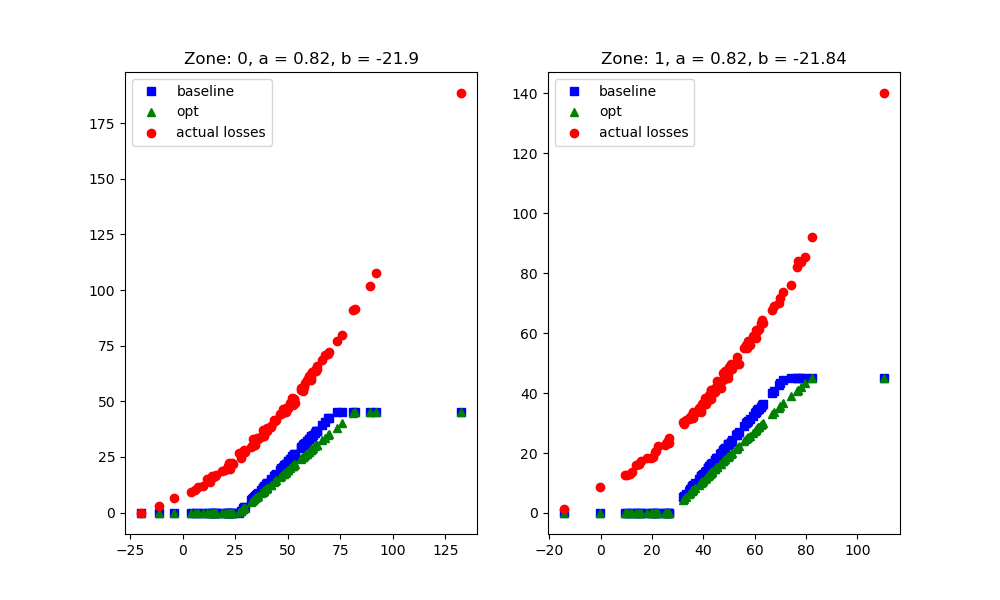
\includegraphics[width=\textwidth]{../../output/figures/Bootstrap/pos_corr_nonlinear_premium.png}
    \end{figure}
\end{frame}

\subsection{Objectives and Constraints}
\begin{frame}{Practitioner Interviews}
\begin{itemize}
   \setlength\itemsep{2em}
    \item We conducted interviews with researchers and practitioners that had implemented index insurance programs in several countries (Malawi, Kenya, Senegal, Thailand, among others) to learn more about the context. 
    \item \textbf{Objective:} minimize risk faced by farmers, maybe minimize probability that wealth drops below a certain threshold.
    \item \textbf{Constraints:} Budget constraints are very important from both demand and supply side.
\end{itemize}    
\end{frame}


\begin{frame}{Risk Measures}
We are interested in minimizing the risk faced by farmers, so we need a measure of this risk. 

\begin{defn}
    For a random variable $z$, representing loss, the $(1-\epsilon)$ Value at Risk $(VaR)$ is given by 
    \begin{align*}
      VaR_{1-\epsilon}(z) := \inf \left \{ t : P(z \leq t) \geq 1-\epsilon \right \}
    \end{align*}
  \end{defn}

  \begin{defn}
    For a random variable $z$, representing loss, the $(1-\epsilon)$ Conditional Value at Risk $(CVaR)$ is given by 
    \begin{align*}
      CVaR_{1-\epsilon}(z) := \mathbb{E}\left [z | z \geq VaR_{1-\epsilon}(z) \right ]
    \end{align*}
  \end{defn}
\end{frame}

\subsection{CVaR Model}
\begin{frame}{Idealized CVaR Model}
\label{ideal-model}
\begin{itemize}
    \item \textbf{Objective:} conditional value at risk of the farmers' loss net of insurance.
    \item  \textbf{Constraint 1:} piecewise linear structure of the contract. 
    \item \textbf{Constraint 2:} budget constraint.
    \item \textbf{Constraint 3:} definition of required capital.
\end{itemize}
 
\begin{align}
        \min_{a,b,\pi, K}  & \quad CVaR_{1-\epsilon}\left ( \ell + \mathbb{E}[I(\theta)] - I(\theta) \right) \notag\\
        \text{s.t.   }I(\theta) &= \min \{ (a\hat{\ell}(\theta) + b)^+,P \} \\
        \mathbb{E}&\left [ I(\theta) \right ] + c_{\kappa} K \leq B \\
        K &= \left( CVaR_{1-\epsilon}\left ( I(\theta) \right ) - \mathbb{E}[I(\theta)] \right) \label{cons-budget}
    \end{align}
\end{frame}

\begin{frame}{Multiple Zone}
    \begin{align}
        \min_{a,b,K} \max_z &\quad CVaR_{1-\epsilon}\left (\ell_z + \mathbb{E}[I_z(\theta_z)] - I_z(\theta_z) \right )\\
        \text{s.t.   } &\quad I_z(\theta_z) = \min \{ (a_z\hat{\ell_z}(\theta_z) + b_z)^+,P_z \} \\
        \mathbb{E} &\left [ \sum_z I_z(\theta_z) \right ] + c_{\kappa} K \leq B\\
        K  &= CVaR_{1-\epsilon_K} \left( \sum_z I_z(\theta_z) \right ) - \mathbb{E}\left [ \sum_z I_z(\theta_z) \right]
      \end{align}
\end{frame}

\begin{frame}{Convex Approximation}

\begin{align}
      \min_{a,b,K} \max_z &\quad CVaR_{1-\epsilon}\left (\ell_z + \mathbb{E}\left[ \overline{I_z}(\theta_z) \right ] - \underline{I_z}(\theta_z) \right )\\
      \text{s.t.   } &\quad \mathbb{E}\left [ \sum_z \overline{I_z}(\theta_z) \right ] + c_{\kappa} K \leq B\\
      K  &= CVaR_{1-\epsilon_K} \left( \sum_z \overline{I_z}(\theta_z) \right ) - \mathbb{E}\left [ \sum_z \underline{I_z}(\theta_z) \right]\\
      \overline{I_z}(\theta_z) &= \max \left \{ 0,a_z\hat{\ell_z}(\theta_z) + b_z\right \} \\
      \underline{I_z}(\theta_z) &= \min \{ a_z\hat{\ell_z}(\theta_z) + b_z, P_z \}
    \end{align}
% \hyperlink{ideal-model}{\beamerbutton{Idealized model}}\\
\hyperlink{convex-approx}{\beamerbutton{Convex approximations}}
\end{frame}

\begin{frame}{LP Reformulation}
\scalebox{0.8}{\parbox{\linewidth}{%
Using the results from \cite{rockafellar2002conditional}, we get: 
\begin{align}
      \min_{a,b,\alpha,\gamma,t,m,K^P} \quad & m\\
      \text{s.t.} \quad t_z &+ \frac{1}{\epsilon} \sum_j p^j \gamma_z^j \leq m, \forall z\\
      \gamma_z^j &\geq \ell^j - \min\left\{(a_z\hat{\ell_z}(\theta_z^j) + b_z), P_z\right\} -t_z, \forall j, \forall z \\
      \gamma_z^j &\geq 0, \forall j, \forall z\\
      B &\geq \frac{1}{N} \sum_j \sum_z \alpha^j_z + c_{\kappa} K\\
      t_K &+ \frac{1}{\epsilon_K} \sum_j p^j \gamma_K^j \leq K+Z\pi_{SQ}\\
      \gamma_K^j &\geq \sum_z \alpha^j_z -t_K, \forall j \\
      \gamma_K^j &\geq 0, \forall j\\
      \alpha^j_z &\geq a_z \hat{\ell_z}(\theta^j_z) + b_z, \forall j, \forall z\\
      \alpha^j_z &\geq 0, \forall j, \forall z
  \end{align}
    }}
\end{frame}

\section{Evaluation}
\begin{frame}[noframenumbering, plain]
    \frametitle{Content}
    \tableofcontents[currentsection,currentsubsection]
\end{frame}
\subsection{Baseline Method}\label{baseline}
\begin{frame}{Baseline Method}
    \begin{itemize}
        \setlength\itemsep{1em}
        \item We compare our method to the method developed in \cite{chantarat2013designing}. This method is the most commonly used in academic publications and is what is used in Kenya's index insurance program. 
        \item A linear regression model is used to predict losses in each insured area. A different model is estimated for each area. Each area normally has multiple villages in it. 
        \item Contracts are of the form: $I(\theta) = \min \left \{ (\hat{\ell}(\theta)-\ell^*)^+,P \right \}$ where $\hat{\ell}(\theta)$ is the predicted loss,  $\ell^*$ is the strike value, and $P$ is the maximum payout. In other words, their contract pays farmers for the full predicted loss beyond a threshold, $\ell^*$. This threshold, $\ell^*$ is the contract's strike value. The strike value is chosen to maximize the correlation of payouts and losses. 
    \end{itemize}
\end{frame}

\subsection{Synthetic Data Evaluation}
\begin{frame}[noframenumbering, plain]
    \frametitle{Content}
    \tableofcontents[currentsection,currentsubsection]
\end{frame}

\begin{frame}{Setup}
    We use the following data generating processes:  
      \begin{itemize}
        \item Linear DGP: $\ell = \beta \theta + \epsilon$
        \item Nonlinear DGP: $\ell = \beta \theta^2 + \epsilon$
      \end{itemize}

    In both cases we have: $\theta \sim \mathcal{N}((5,5),\Sigma), \beta = diag(1.5,1.5), \epsilon \sim \mathcal{N}(0,I)$. \\~~\\
    With each data generating process, we test the following scenarios: 
    \begin{itemize}
          \item \textbf{No correlation case:} $corr(\theta_1,\theta_2) = 0$
          \item \textbf{Positive correlation case:} $corr(\theta_1,\theta_2) = 0.8$
          \item \textbf{Negative correlation case:} $corr(\theta_1,\theta_2) = 0.8$
      \end{itemize}
\end{frame}

\begin{frame}{Simulation Details}
In each simulation we: 
    \begin{enumerate}
        \item Generate training and test samples, samples will be of the form $\left \{\ell^i_1,\theta^i_1, \ell^i_2, \theta^i_2 \right \}_{i=1}^N$ where $\ell$ is loss and $\theta$ is the predictor. 
        \item Train linear prediction model. We run $\ell = \beta_0 + \beta_1\theta +\epsilon$. Use model to generate predictions $\hat{\ell}(\theta)$ for training and test data. 
        \item Use training data and model predictions to design contracts using both methods.  
        \item Given test data and predicted losses, calculate payouts from both contracts. 
        \item Calculate performance metrics on test data. 
        \end{enumerate}
We run this 500 times for each scenario. We report the mean and $95 \%$ confidence intervals of each performance metric across the 500 simulations.
\end{frame}

\begin{frame}{Performance Metrics}
    For each sample in the test set, we calculate the net loss, $\Delta \ell_z^i \triangleq  \ell^i_z + \pi_z - I_z(\theta^i_z)$. 
    \begin{itemize}
        \item \textbf{Maximum CVaR:} This is the expected value of the net loss given the loss is above a certain threshold. $CVaR_z = \mathbb{E}\left [ \Delta \ell_z | \ell_z \geq VaR_{0.8} (\ell_z) \right ]$.
        \item \textbf{Maximum VaR:} This the $80^{th}$ quantile of the distribution of the net loss. 
        \item \textbf{Maximum Semi-variance}: This is the variance conditional on the loss being beyond a certain threshold. $\frac{1}{N-1}\sum_i (\Delta \ell_z^i - \overline{\ell})^2 \mathbbm{1} \{\ell_z > \overline{\ell_z}\}$ 
        \item \textbf{$|VaR_2 - VaR_1|$:} Absolute value of the difference betweent the $VaR$ of the two zones. 
        \item \textbf{Required Capital:} $K(I(\theta)) = CVaR_{1-\epsilon_P}(\sum_z I_z(\theta)) - \mathbb{E}[\sum_z I_z(\theta)]$. 
        \item \textbf{Average Cost:} We define this to be $\frac{1}{N}\sum_{i=1}^N \sum_z I_z(\theta^i_z) + c_{\kappa} K$. This is the empirical average of the cost of the insurance in every scenario in the test set plus the cost of capital
    \end{itemize}
\end{frame}

\begin{frame}{Summary of Results: Correctly Specified Model}
Our model outperforms or matches the performance of the baseline contracts in the following areas: 
\begin{itemize}
%   \setlength\itemsep{2em}
    \item \textbf{Maximum Value at Risk:} the value at risk of the worst off zone is lower under our contracts, usually by about $5-6\%$.
    \item \textbf{Equity:} the difference in the value at risk of the two zones is lower under our contracts.  
    
    \item \textbf{Maximum Semi-Variance} the variance conditional on loss exceeding a certain threshold is lower in our model, usually by about $20\%$.
    
    \item \textbf{Required Capital:} The contracts designed by our model consistently require less capital to fund than the baseline, $12-15\%$ less capital. 
\end{itemize}
\end{frame}

\begin{frame}[noframenumbering, plain]{Results: Correctly Specified Prediction Model}
\fontsize{6.5pt}{8pt}\selectfont
\begin{table}
\subcaptionbox{No correlation}{
    \begin{tabular}{ccccccc}
        \toprule
   Model &     Max CVaR &      Max VaR &    Max SemiVar & $|VaR_2 - VaR_1|$ & Required Capital & Average Cost \\
\midrule
Baseline &         6.23 &         6.35 &          19.72 &              0.87 &             7.04 &         6.11 \\
         &  [6.17, 6.3] & [6.29, 6.41] & [19.26, 20.17] &      [0.81, 0.93] &     [6.94, 7.14] &  [6.02, 6.2] \\
     Opt &         6.18 &         5.98 &          14.78 &              0.21 &             6.12 &         6.08 \\
         & [6.13, 6.24] & [5.93, 6.02] & [14.38, 15.19] &       [0.2, 0.23] &     [6.03, 6.21] & [5.99, 6.17] \\
    Diff &         0.05 &         0.37 &           4.93 &              0.66 &             0.92 &         0.03 \\
         & [0.02, 0.08] &  [0.34, 0.4] &   [4.66, 5.21] &       [0.6, 0.72] &     [0.88, 0.95] & [0.02, 0.03] \\
\bottomrule
        \end{tabular}}

\subcaptionbox{Positive correlation}{
    \begin{tabular}{ccccccc}
        \toprule
   Model &      Max CVaR &      Max VaR &    Max SemiVar & $|VaR_2 - VaR_1|$ & Required Capital & Average Cost \\
\midrule
Baseline &          6.19 &         6.28 &          19.44 &              0.77 &             9.18 &         6.45 \\
         &  [6.12, 6.26] & [6.22, 6.34] & [18.98, 19.91] &      [0.72, 0.83] &     [9.09, 9.28] & [6.36, 6.54] \\
     Opt &          6.21 &         5.94 &          14.24 &              0.19 &             7.81 &         6.41 \\
         &  [6.15, 6.26] & [5.89, 5.99] & [13.84, 14.65] &      [0.18, 0.21] &      [7.7, 7.91] &  [6.32, 6.5] \\
    Diff &         -0.02 &         0.34 &            5.2 &              0.58 &             1.38 &         0.04 \\
         & [-0.05, 0.01] & [0.31, 0.37] &   [4.95, 5.46] &      [0.52, 0.63] &     [1.33, 1.43] & [0.03, 0.05] \\
\bottomrule
        \end{tabular}}

\end{table}
\end{frame}

\begin{frame}[noframenumbering, plain]{Results: Correctly Specified Prediction Model}
\fontsize{6.5pt}{8pt}\selectfont
\begin{table}
    \centering 
    \begin{tabular}{ccccccc}
        \toprule
           Model &     Max CVaR &      Max VaR &    Max SemiVar & $|VaR_2 - VaR_1|$ & Required Capital & Average Cost \\
        \midrule
        Baseline &         6.19 &          6.3 &          19.72 &              0.85 &             3.33 &         5.56 \\
                 & [6.13, 6.26] & [6.24, 6.36] & [19.27, 20.17] &       [0.79, 0.9] &     [3.28, 3.38] & [5.48, 5.64] \\
             Opt &         6.11 &         5.98 &          15.09 &              0.22 &             2.91 &         5.53 \\
                 & [6.06, 6.17] & [5.93, 6.02] &  [14.68, 15.5] &       [0.2, 0.23] &     [2.86, 2.95] & [5.45, 5.61] \\
            Diff &         0.08 &         0.32 &           4.63 &              0.63 &             0.42 &         0.04 \\
                 & [0.05, 0.11] & [0.29, 0.35] &    [4.35, 4.9] &      [0.57, 0.69] &     [0.39, 0.45] & [0.03, 0.04] \\
        \bottomrule
        \end{tabular}
        \caption{Negative correlation}
\end{table}
\end{frame}

\begin{frame}{Summary of Results: Misspecified Model}
    A fair comparison is harder in this case because it becomes harder to enforce the budget constraint, and the models end up having different costs. Our model generally does better on the following metrics: 
    \begin{itemize}
      \setlength\itemsep{1em}
        
      \item \textbf{Maximum Semi-Variance} the variance conditional on loss exceeding a certain threshold is lower in our model, usually by about $20\%$.
        
        \item \textbf{Required Capital:} The contracts designed by our model generally require less capital to fund than the baseline, $12-15\%$ less capital. 
        \item \textbf{Average Cost}: The contracts designed by our model tend to be $6-10\%$ less costly. 
    \end{itemize}
    However, it does worse on all other metrics. We can make it competitive using a heuristic reallocation policy. 
    \end{frame}

\begin{frame}[noframenumbering, plain]{Results: Misspecified Prediction Model}
    \fontsize{6.5pt}{8pt}\selectfont
    \begin{table}
    \subcaptionbox{No correlation}{
        \begin{tabular}{ccccccc}
            \toprule
            Model &       Max CVaR &        Max VaR &      Max SemiVar & $|VaR_2 - VaR_1|$ & Required Capital &   Average Cost \\
         \midrule
         Baseline &          35.54 &          27.43 &           820.02 &              2.25 &             53.1 &          40.94 \\
                  & [35.28, 35.79] &  [27.3, 27.56] &  [806.9, 833.15] &      [2.07, 2.43] &   [52.67, 53.52] &  [40.69, 41.2] \\
              Opt &          38.67 &          30.61 &           628.58 &              2.41 &            50.87 &          38.31 \\
                  &  [38.44, 38.9] & [30.45, 30.76] & [616.93, 640.23] &      [2.25, 2.58] &   [50.33, 51.41] & [38.06, 38.56] \\
             Diff &          -3.13 &          -3.18 &           191.44 &             -0.16 &             2.23 &           2.63 \\
                  & [-3.25, -3.01] & [-3.32, -3.04] & [184.69, 198.19] &     [-0.39, 0.06] &      [1.95, 2.5] &   [2.55, 2.72] \\
         \bottomrule
            \end{tabular}}
    
    \subcaptionbox{Positive correlation}{
        \begin{tabular}{ccccccc}
            \toprule
            Model &       Max CVaR &        Max VaR &      Max SemiVar & $|VaR_2 - VaR_1|$ & Required Capital &   Average Cost \\
         \midrule
         Baseline &          34.97 &          27.15 &           817.11 &              1.73 &            56.97 &          41.51 \\
                  & [34.69, 35.25] & [27.02, 27.29] & [803.66, 830.55] &      [1.58, 1.87] &   [56.67, 57.27] & [41.26, 41.77] \\
              Opt &           39.9 &           32.2 &           521.22 &               1.5 &            60.61 &          37.17 \\
                  & [39.63, 40.16] & [32.03, 32.37] & [510.86, 531.58] &       [1.39, 1.6] &    [60.3, 60.91] & [36.94, 37.41] \\
             Diff &          -4.93 &          -5.04 &           295.88 &              0.23 &            -3.64 &           4.34 \\
                  &  [-5.05, -4.8] &  [-5.19, -4.9] & [288.47, 303.29] &       [0.06, 0.4] &   [-3.88, -3.39] &   [4.23, 4.45] \\
         \bottomrule
            \end{tabular}}
    
    \end{table}
    \end{frame}
    

% \begin{frame}{Relationships between parameters and correlation}
% \begin{itemize}
%     \item Positive correlation leads to smaller but more frequent payouts
%     \item Negative correlation leads to less frequent but more aggressive payouts
% \end{itemize}
% \begin{figure}
% \centering
%   \begin{subfigure}[b]{0.45\textwidth}
%     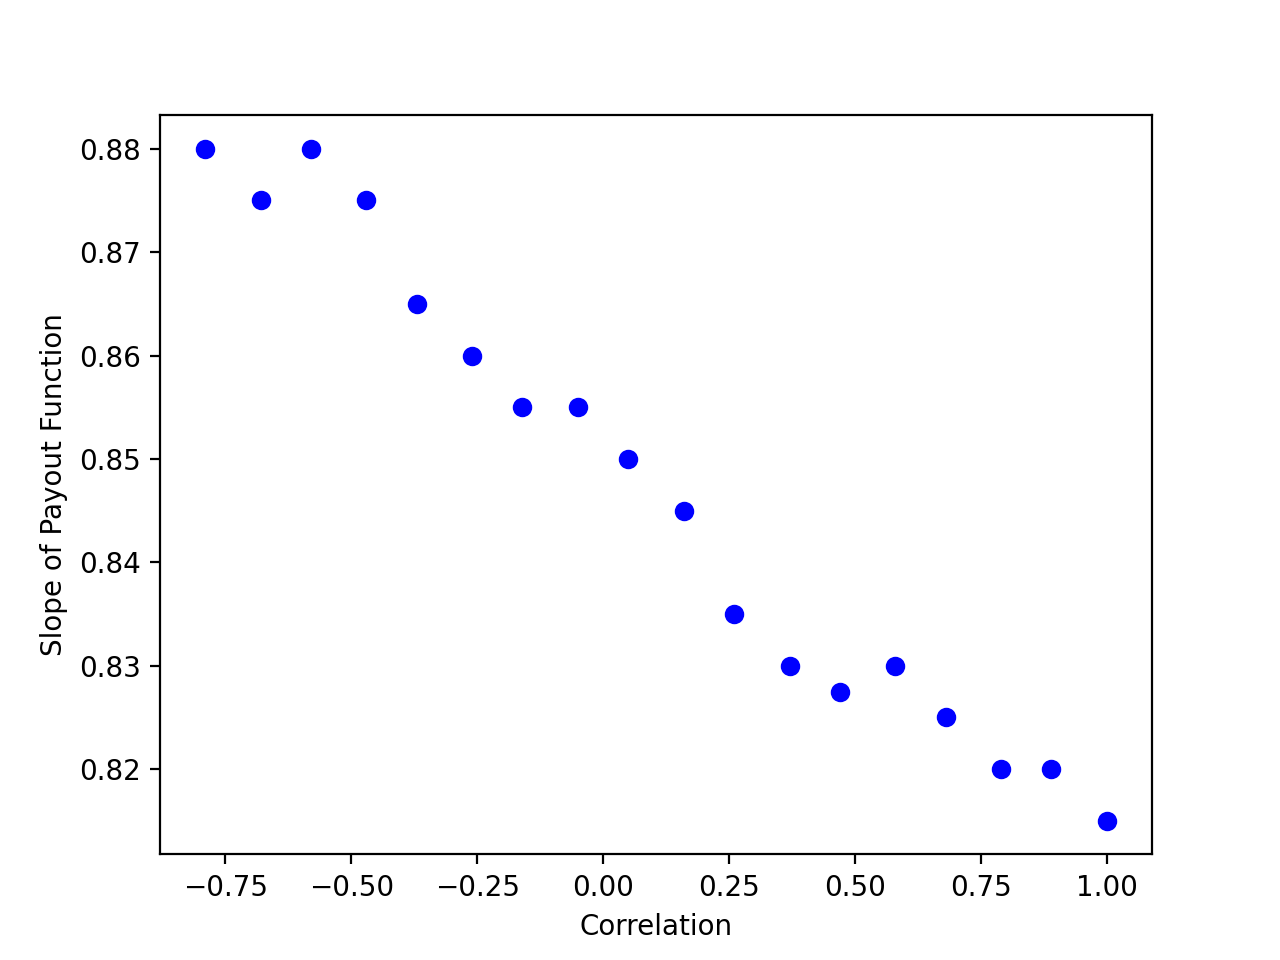
\includegraphics[width=\textwidth]{slope_vs_corr.png}
%     \caption{Slope of payout function vs correlation}
%     \label{fig:f1}
%   \end{subfigure}
%  \hfill
%   \begin{subfigure}[b]{0.45\textwidth}
%     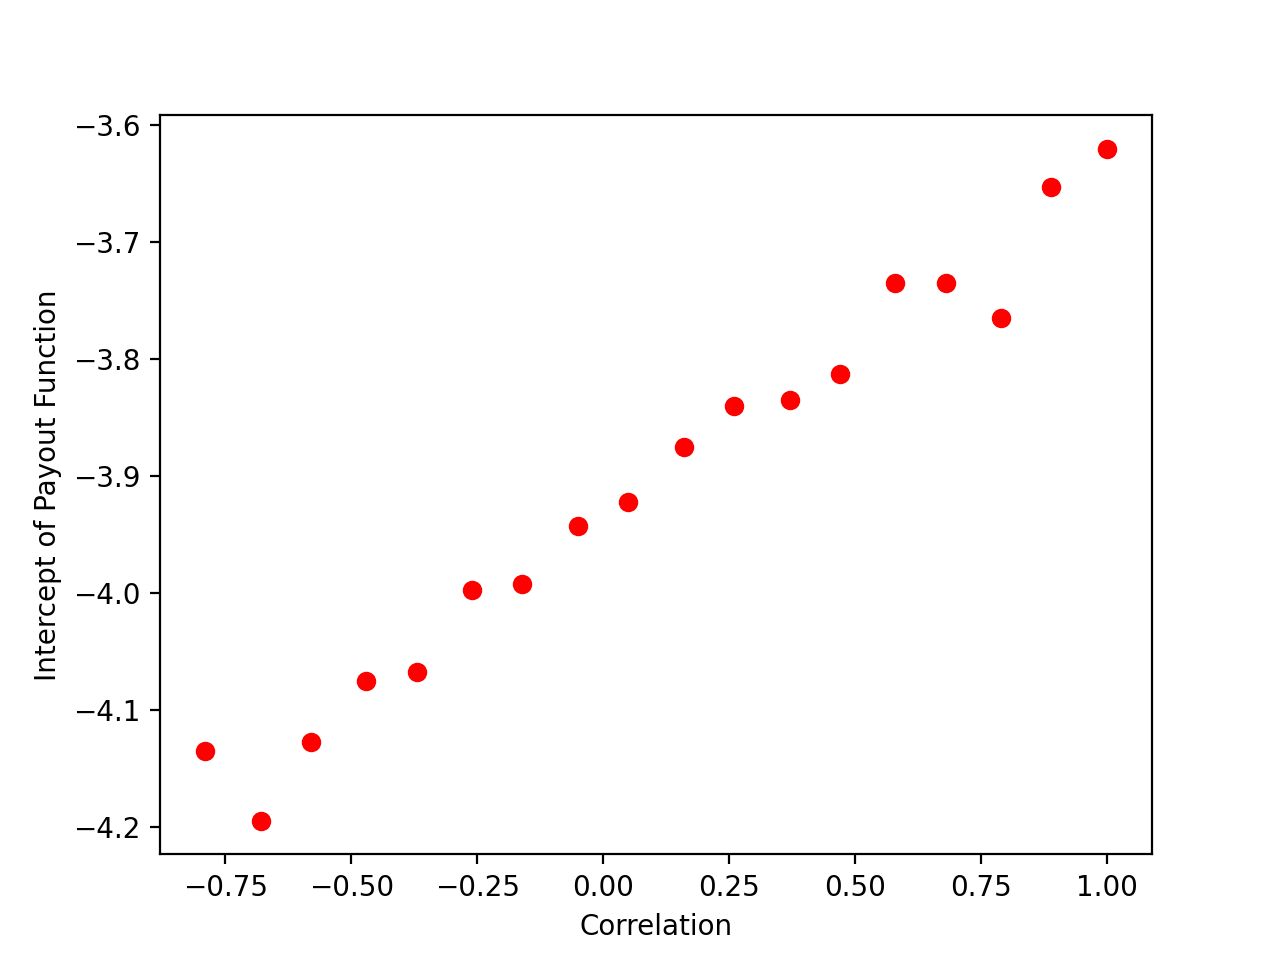
\includegraphics[width=\textwidth]{intercept_vs_corr.png}
%     \caption{Intercept of payout function vs correlation}
%     \label{fig:f2}
%   \end{subfigure}
%   \caption{Relationship between parameters and correlation}
% \end{figure}
    
% \end{frame}



\subsection{Kenya Pastoralist Data}
\begin{frame}[noframenumbering, plain]
    \frametitle{Content}
    \tableofcontents[currentsection,currentsubsection]
\end{frame}

\begin{frame}{Data Sources}
\begin{itemize}
    \setlength\itemsep{1em}
    \item \textbf{NDVI Data:} The Normalized Difference Vegetation Index (NDVI) is a satellite-based indicator of the amount and health of vegetation. We use NDVI data for Kenya between 2000-2015. There are $\sim 23,000,000$ observations per time period, and 365 time periods.
    \item \textbf{Kenya Household Survey Data:} This survey was conducted as part of the development of the Index based livestock insurance (IBLI) program in northern Kenya.  This dataset has information on household location, livestock levels and changes for each month in 2010-2013. There are 900 households in this dataset. 
    \item \textbf{Kenya Geospatial Data:} This dataset contains the geospatial boundaries of larger villages in Kenya. 
\end{itemize}
\end{frame}

\begin{frame}{Data Creation}
\begin{enumerate}
   \item Data for prediction model
   \begin{enumerate}
       \item NDVI Data
       \begin{enumerate}
        %    \item Change NDVI data coordinates to standard coordinates
           \item Use geospatial information to merge NDVI data with village geospatial data. 
           \item For each village, you now have many NDVI values. Use this to calculate village level features for relevant time periods. 
           \item \textbf{Outcome:} data set with village level NDVI features across time.
       \end{enumerate}
       \item Survey Data
       \begin{enumerate}
           \item Merge survey data with Kenya geospatial data. 
           \item Calculate herd mortality for each village in each season. 
           \item \textbf{Outcome:} data set with village level herd mortality across time
       \end{enumerate}
       \item Merge two datasets at the village by season level.
   \end{enumerate}
   \item Train prediction model using data from previous step. 
    \item Add model predictions to household survey data 
\end{enumerate}
% \begin{enumerate}
%     \item Calculate NDVI metrics for each village in each season. These metrics will be the features for our predictive model. 
%     \item Use household data to calculate average livestock mortality in each village in each season. 
%     \item Merge the two resulting datasets to create a dataset for regression.
%     \item Train prediction model for each cluster and use this model to predict herd mortality at the village level. 
%     \item Add model predictions to household data. 
% \end{enumerate}   
\end{frame}

\begin{frame}{Evaluation Procedure}
We use leave one out cross validation to evaluate our method. In each iteration, we leave out one year of data for testing.
\begin{enumerate}
    \item Split regression data and household survey data into training/test set
    \item Train prediction model on training data
    \item Use model to calculate village level predicted losses, add this to household training data
    \item Calculate insurance contracts based on the training data using both methods.
    \item Use prediction model to calculate village level predicted losses on the test set. 
    \item Calculate insurance payouts on test data.
\end{enumerate}
\end{frame}

\begin{frame}{Results}
The insurance contracts developed by our model provide slightly better protection at a much lower cost. The cost of our contracts is $9\%$ lower, and the cost of capital is $13\%$ lower. 
\begin{table}[]
\small
    \centering
    \begin{tabular}{lrrrr}
\toprule
    Model &  Max VaR &  $|VaR_2 - VaR_1|$ &  Required Capital &  Average Cost \\
\midrule
 Baseline &     1303 &               1316 &           3014405 &          6449 \\
      Opt &     1286 &               1361 &           2626260 &          5864 \\
\bottomrule
\end{tabular}
    \caption{Results using Kenya household data}
    
\end{table}
\end{frame}

\section{Conclusion and Next Steps}
\subsection{Conclusions}
\begin{frame}{Conclusions}
    \begin{itemize}
    \setlength\itemsep{2em}
        \item In some cases, the contracts designed by our model are able to offer better protection at a similar costs, or comparable protection at lower costs than the baseline method. 
        \item It outperforms the baseline when the prediction model is correclty specified and on the Kenyan pastoralist data. 
        \item Our method is more cost effective because it takes into account spatial correlations between  areas and the costs of capital requirements. Thus, the model makes better trade offs between costs and coverage than the baseline method. 
        
    \end{itemize}
\end{frame}

\subsection{Next Steps}
\begin{frame}{Next Steps}
\begin{itemize}
\setlength\itemsep{2em}
    \item We are working with practitioners to improve the model and possibly test it in practice.
    \item We are working with the Bank of Thailand on the implementation of their satellite-based index insurance program. 
    \item We are also talking to the International Research Institute for Climate and Society at Columbia, they have worked on the implementation of numerous index insurance programs in Africa.   
\end{itemize}
\end{frame}

\begin{frame}[noframenumbering, plain]{References}
\printbibliography
\end{frame}

\begin{frame}[noframenumbering, plain]{Idealized CVaR Model}
% \label{ideal-model}
\begin{itemize}
    \item \textbf{Objective:} conditional value at risk of the farmers' loss net of insurance.
    \item  \textbf{Constraint 1:} piecewise linear structure of the contract. 
    \item \textbf{Constraint 2:} budget constraint.
    \item \textbf{Constraint 3:} definition of required capital.
\end{itemize}
 
\begin{align}
        \min_{a,b,\pi, K}  & \quad CVaR_{1-\epsilon}\left ( \ell - I(\theta) \right) \notag\\
        \text{s.t.   }I(\theta) &= \min \{ (a\hat{\ell}(\theta) + b)^+,P \} \\
        \mathbb{E}\left [ I(\theta) \right ] &+ c_{\kappa} K \leq B \\
        K &= \left( CVaR_{1-\epsilon}\left ( I(\theta) \right ) - \mathbb{E}[I(\theta)] \right) \label{cons-budget}
    \end{align}
\end{frame}

\begin{frame}[noframenumbering, plain]{The problem is non-convex, so we need convex approximations}
\label{convex-approx}
We use the following approximations of $I(\theta)$ to make the problem convex: 
\begin{align*}
    \overline{I(\theta)} &\triangleq \max \left \{ 0,a\hat{\ell}(\theta) + b\right \} \\
    \underline{I(\theta)} &\triangleq \min \{ a\hat{\ell}(\theta) + b,K \}
\end{align*}
\begin{itemize}
    \item Note that $\overline{I(\theta)} \geq I(\theta)$ and $\overline{I(\theta)}$ is convex. Conversely, $\underline{I(\theta)} \leq I(\theta)$ and $\underline{I(\theta)}$ is concave. 
    \item We replace $I(\theta)$ with either $\overline{I(\theta)}$ or $\underline{I(\theta)}$ where necessary to obtain conservative and convex approximations. 
    \item We also need approximations or proxies for $E[I(\theta)]$ in constraint \ref{cons-budget}. We use $\pi_{SQ} = E[I_{SQ}(\theta)]$, where $I_{SQ}$ is the contract designed using the status quo method, as a proxy for $E[I(\theta)]$ in constraint \ref{cons-budget}.
\end{itemize}
\end{frame}

\begin{frame}[noframenumbering, plain]{Insights: Relationships between parameters and epsilon}
\label{eps-relationship}
As $\epsilon$ gets smaller, the slope increases and the function shifts to the right. 
\begin{figure}
\centering
  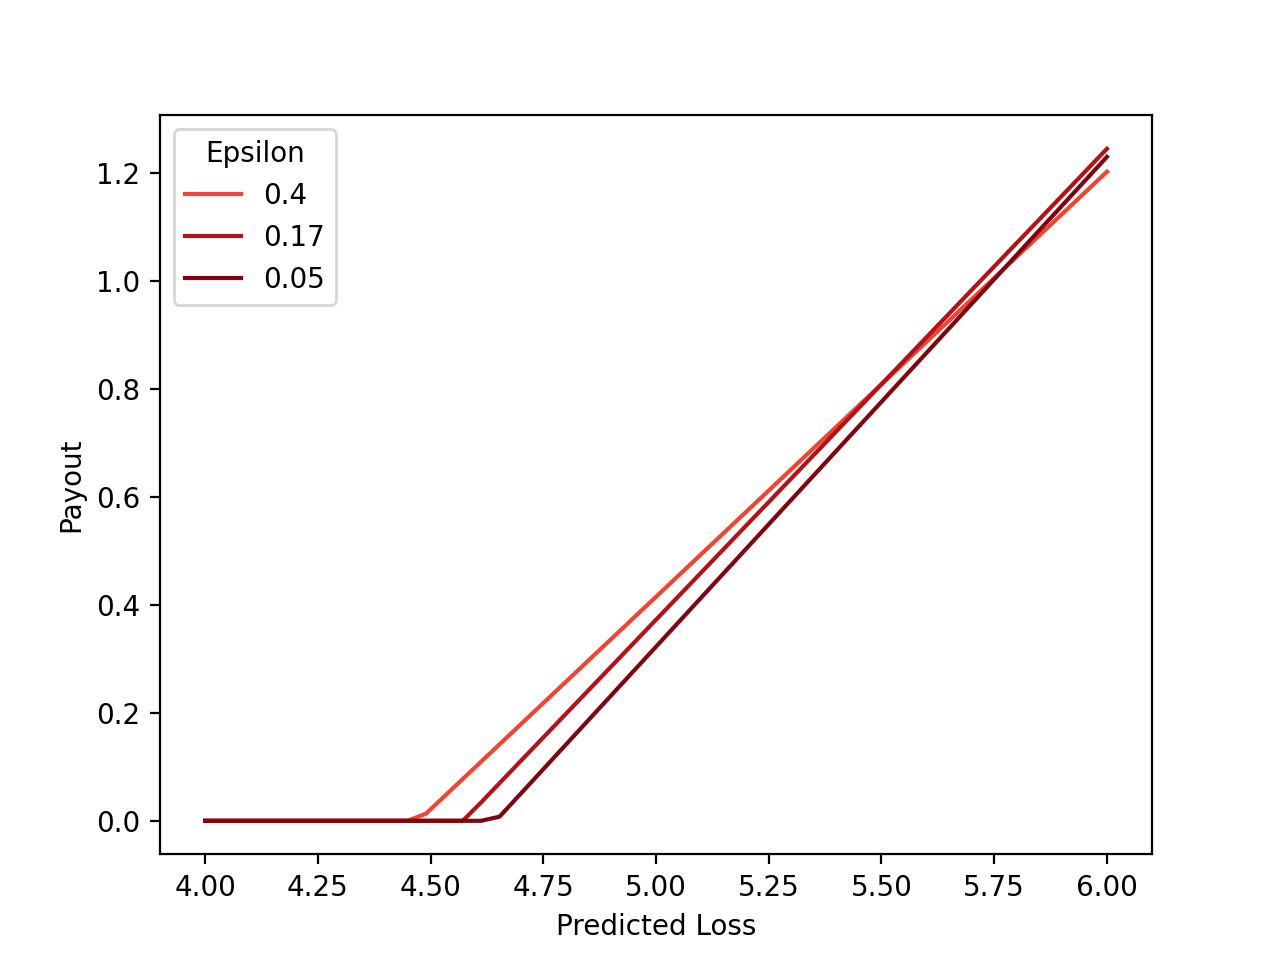
\includegraphics[width=0.65\textwidth, height=0.5\textwidth]{payout_vs_epsilon.png}
\end{figure}
    
\end{frame}

\begin{frame}[noframenumbering, plain]{Results: Misspecified Prediction Model}
\label{misspec-results}
\fontsize{6.5pt}{8pt}\selectfont
\begin{table}
\subcaptionbox{No correlation}{
\begin{tabular}{ccccc}
\toprule
   Model &        Max VaR & $|VaR_2 - VaR_1|$ & Required Capital &   Average Cost \\
\midrule
Baseline &          27.42 &              1.65 &            53.85 &          40.73 \\
         & [25.13, 29.57] &      [0.16, 5.56] &   [44.81, 59.88] & [36.06, 45.83] \\
     Opt &          27.41 &              1.96 &            49.97 &          40.36 \\
         & [24.53, 29.83] &       [0.15, 5.6] &   [42.87, 58.53] &  [35.52, 45.5] \\
\bottomrule
\end{tabular}}

\subcaptionbox{Positive correlation}{
\begin{tabular}{ccccc}
\toprule
   Model &        Max VaR & $|VaR_2 - VaR_1|$ & Required Capital &   Average Cost \\
\midrule
Baseline &          27.16 &              1.23 &             57.1 &          41.36 \\
         &  [24.7, 29.62] &       [0.1, 5.05] &    [51.16, 62.9] & [36.24, 46.52] \\
     Opt &          27.71 &               1.1 &            56.51 &          41.31 \\
         & [24.91, 30.31] &      [0.09, 3.62] &   [50.92, 62.26] & [35.98, 46.82] \\
\bottomrule
\end{tabular}}

\subcaptionbox{Negative correlation}{
\begin{tabular}{ccccc}
\toprule
   Model &        Max VaR & $|VaR_2 - VaR_1|$ & Required Capital &   Average Cost \\
\midrule
Baseline &          27.52 &               1.9 &             25.2 &          36.42 \\
         & [25.09, 29.69] &       [0.17, 6.0] &   [17.99, 36.35] & [33.13, 41.88] \\
     Opt &          27.39 &              1.84 &            26.77 &          36.67 \\
         & [24.33, 29.71] &      [0.16, 5.49] &    [18.17, 37.5] & [33.21, 42.03] \\
\bottomrule
\end{tabular}
}
\end{table}
\end{frame}

\end{document}